\documentclass[11pt,a4paper]{article}
\usepackage[utf8]{inputenc}
\usepackage[T1]{fontenc}
\usepackage{amsmath,amssymb,amsfonts}
\usepackage{graphicx}
\usepackage{booktabs}
\usepackage{multirow}
\usepackage{hyperref}
\usepackage{cleveref}
\usepackage{xcolor}
\usepackage{microtype}
\usepackage[margin=1in]{geometry}
\usepackage{natbib}
\usepackage{subcaption}
\usepackage{tikz}
\usetikzlibrary{positioning,arrows.meta,shapes.geometric,fit,calc,backgrounds,decorations.pathreplacing}

\hypersetup{colorlinks=true,linkcolor=blue,citecolor=blue,urlcolor=blue}

\title{Hybrid MoE: Integrating Deterministic Computation Experts \\
into Sparse Mixture-of-Experts Transformers}

\author{
Pavan Kumar Kotha \\
Independent Researcher \\
\texttt{kothapavan1998@gmail.com}
}

\date{}

\begin{document}
\maketitle

\begin{abstract}
Large language models struggle with deterministic numerical computation,
a critical limitation in domains like financial underwriting where exact
calculations are non-negotiable. We introduce \textbf{Hybrid MoE}, a
novel architecture that integrates deterministic Python functions as
first-class experts within a sparse Mixture-of-Experts (MoE) transformer's
routing mechanism. Each deterministic expert consists of three stages:
(1)~a learned extraction MLP that recovers function arguments from the
hidden state, (2)~an exact deterministic computation (e.g., DSCR = NOI /
Annual Debt Service), and (3)~a learned projection that re-injects the
result into the residual stream. Using OpenAI's gpt-oss-20b (21B parameters,
32 experts per layer) as the base model, we extend the router to select
from 36~experts (32~frozen neural + 4~deterministic) with
${\sim}$1.5M parameters per extraction probe (${\sim}$12M total). On a commercial real estate underwriting benchmark
(3{,}000 training, 200 evaluation scenarios), we show that:
(i)~financial values encoded in hidden states can be recovered with
5-fold cross-validated $R^2 = 0.98 \pm 0.002$ using mean-pooled
representations, (ii)~the routing signal achieves 100\% accuracy in
detecting computation-requiring inputs, and (iii)~Hybrid MoE produces
results \textbf{173$\times$ faster} (40\,ms vs.\ 7{,}000\,ms) than
single-sample generation. Hybrid MoE achieves 60--87\% accuracy within
20\% error across all four experts with \emph{guaranteed coverage}
($N{=}200$ for every metric), whereas generation-based baselines parse
answers for only 1--94\% of scenarios depending on metric and prompt
format. We analyze which numerical quantities are extractable from MoE
hidden states, identify extraction quality as the primary bottleneck,
and show that 5-fold cross-validated ensembles resolve probe training
instability on small datasets.
\end{abstract}

\section{Introduction}
\label{sec:intro}

Large language models (LLMs) have achieved remarkable capabilities across
language understanding, generation, and reasoning tasks. However, they
fundamentally struggle with \emph{deterministic numerical computation}
, specifically the reliable execution of mathematical formulas that require exact
arithmetic on multi-digit numbers
\citep{dziri2023faith}. This limitation is
particularly consequential in professional domains such as financial
underwriting, where metrics like the Debt Service Coverage Ratio (DSCR)
or Loan-to-Value (LTV) must be computed with precision sufficient for
legal and regulatory compliance.

Current approaches to equipping LLMs with computational ability fall into
three categories, each with significant drawbacks:

\begin{itemize}
\item \textbf{External tool calling} (ReAct \citep{yao2023react},
Toolformer \citep{schick2023toolformer}): Each computation requires a
separate inference pass and API round-trip. A chained calculation like
computing Annual Debt Service and then DSCR requires 2+ full
generation cycles.
\item \textbf{Chain-of-Thought prompting} \citep{wei2022chain}: The model
performs arithmetic in its generated text. This works for simple
calculations but systematically fails on six-or-more-digit numbers
and multi-step compound formulas \citep{dziri2023faith}.
\item \textbf{Tool tokens} (ToolkenGPT \citep{hao2023toolkengpt}): Tools
are represented as special vocabulary tokens. Argument extraction
relies on prompting rather than learned representations, and
integration occurs at the language model head rather than within the
model's representational layers.
\end{itemize}

We observe that sparse Mixture-of-Experts (MoE) architectures
\citep{shazeer2017outrageously,fedus2022switch,jiang2024mixtral} provide
a natural mechanism for integrating heterogeneous computation: the expert
routing mechanism already selects specialized processing modules on a
per-token basis. If some of these experts were deterministic functions
instead of neural feed-forward networks, the router could learn
\emph{when} to invoke exact computation and the model could perform it
\emph{within a single forward pass}.

We introduce \textbf{Hybrid MoE}, an architecture that extends the
expert pool of an MoE transformer with \emph{deterministic computation
experts}, which are non-neural expert modules that execute exact domain
computations. Each deterministic expert comprises three stages:
\begin{enumerate}
\item A \textbf{parameter extraction MLP} (learned) that reads the hidden
state and outputs the numerical arguments required by the target
function.
\item A \textbf{deterministic computation} (exact) that executes the
domain formula as a standard PyTorch function, maintaining
differentiability through autograd.
\item A \textbf{result projection MLP} (learned) that maps the scalar
output back to the model's hidden dimension for re-injection into
the residual stream.
\end{enumerate}

We implement Hybrid MoE on top of OpenAI's gpt-oss-20b, a 21-billion
parameter MoE model with 32 experts per layer and top-4 routing. We
extend the router from 32 to 36 experts by adding 4 deterministic
experts for commercial real estate (CRE) underwriting metrics:
DSCR, LTV, Capitalization Rate, and Debt Yield. The entire modification
adds approximately 1.5 million parameters per extraction probe
(approximately 12 million total) while the base model remains fully
frozen.

Our contributions are:
\begin{enumerate}
\item \textbf{A novel heterogeneous expert architecture} that integrates
deterministic Python functions as first-class experts in MoE
routing, enabling exact computation within a single forward pass
(\Cref{sec:method}).
\item \textbf{Empirical demonstration} that financial numerical values
can be recovered from transformer hidden states with 5-fold
cross-validated $R^2$ up to 0.98, and that a learned router
achieves 100\% accuracy in detecting computation-requiring inputs
(\Cref{sec:experiments}).
\item \textbf{A 173$\times$ speedup} over generation-based methods
(40\,ms vs.\ 7{,}000\,ms per scenario), achieving 60--87\%
accuracy within 20\% error across all four experts with guaranteed
coverage ($N{=}200$), while generation baselines produce parseable
answers for only 1--94\% of scenarios (\Cref{sec:experiments}).
\item \textbf{Analysis of extraction robustness}, demonstrating that
probe training instability (not hidden state quality) causes
extraction failures on small datasets, and that 5-fold CV
ensembles resolve this (\Cref{sec:analysis}).
\end{enumerate}

\section{Related Work}
\label{sec:related}

\paragraph{Sparse Mixture-of-Experts.}
MoE models route each token to a subset of experts, achieving
sub-linear inference cost relative to total parameters
\citep{shazeer2017outrageously,lepikhin2021gshard}. Switch Transformer
\citep{fedus2022switch} simplified routing to top-1 selection.
Mixtral \citep{jiang2024mixtral} demonstrated strong open-weight MoE
models with top-2 routing across 8 experts. DeepSeek-V2
\citep{deepseekai2024deepseekv2} introduced fine-grained experts and
shared expert isolation. Our base model, gpt-oss-20b, uses 32 experts
per layer with top-4 routing and sigmoid-normalized weights. To our knowledge, all prior MoE work uses exclusively neural or
trivial (zero/copy) experts; we introduce \emph{deterministic
computation} experts that execute exact domain functions.

\paragraph{MoE Expert Expansion.}
Several works have added experts to existing MoE models post-training.
Sparse Upcycling \citep{komatsuzaki2023sparse} converts dense models
to MoE by duplicating FFN layers as experts. Branch-Train-Merge
\citep{li2022branch} trains expert modules independently. MoE++
\citep{jin2024moepp} introduces heterogeneous expert types (zero
experts, copy experts) but these perform trivial operations. Nexus
\citep{gritsch2024nexus} adds task-specialized neural experts with
adaptive routing from domain embeddings. All of these add \emph{neural} experts.
Our deterministic experts are a fundamentally new class: they execute
exact symbolic computation rather than learned approximations.

\paragraph{Tool-Augmented Language Models.}
Toolformer \citep{schick2023toolformer} teaches models to insert API
calls into generated text via self-supervised learning. ReAct
\citep{yao2023react} interleaves reasoning and action traces for
multi-step tool use. ToolkenGPT \citep{hao2023toolkengpt} represents
tools as special vocabulary tokens, enabling tool invocation through
standard next-token prediction. Gorilla \citep{patil2023gorilla}
fine-tunes models on API documentation. These approaches share a common
limitation: tool execution is \emph{external} to the model, requiring
separate inference passes, API calls, or decoding steps. Hybrid MoE
embeds computation \emph{inside} the forward pass through the MoE
routing mechanism.

\paragraph{In-Model Arithmetic and Neurosymbolic Integration.}
The broader vision of combining neural and symbolic computation has a
long history \citep{garcez2019neural}. Two recent works are closely
related to ours. OccamLLM \citep{deleo2024occamllm} uses LLM hidden
states to control a symbolic architecture (OccamNet) that performs
exact arithmetic operations ($+, -, \times, \div, \sin$, etc.) in a
single autoregressive step, achieving 100\% accuracy on individual
operations. IGC \citep{dietz2025igc} integrates a gated calculator
directly into the LLM forward pass, achieving 98--99\% on the BigBench
Arithmetic benchmark without external tools. Both demonstrate that
hidden states contain sufficient information to drive exact computation.
Our work differs from these approaches in using \emph{MoE routing} for
dispatch: rather than adding a separate module or gating mechanism, we
extend the existing expert routing to naturally select between neural and
deterministic experts, which avoids introducing new architectural
components and allows the model to decide when computation is needed
through the same mechanism it already uses for expert selection.
Additional related work includes neural module networks
\citep{andreas2016neural} and dual-system neuro-symbolic approaches
\citep{nye2021improving,baydin2018automatic}.

\paragraph{Numerical Representations in LLMs.}
Understanding how transformers encode numbers is an active area.
\citet{wallace2019nlp} showed that MLPs can probe word embeddings for
numerical magnitudes. \citet{geva2023dissecting} demonstrated that
factual information is stored in specific feed-forward neurons.
\citet{chen2024states} found that LLMs develop ``implicit discrete
state representations'' for numerical reasoning, though these are ``far
from lossless.'' \citet{bai2025numbers} showed that LLMs encode number
values linearly in hidden states, recovering log-magnitudes with
${\sim}2.3\%$ error via linear probes. Most relevantly,
\citet{razeghi2022impact} showed that numerical reasoning accuracy
correlates with the frequency of specific numbers in pretraining data.
Our extraction experiments extend this line of work to domain-specific
financial values (NOI, loan amounts, property values), showing that
mean-pooled representations at middle layers encode these quantities
with $R^2$ up to 0.98.

\section{Method}
\label{sec:method}

\begin{figure*}[t]
\centering
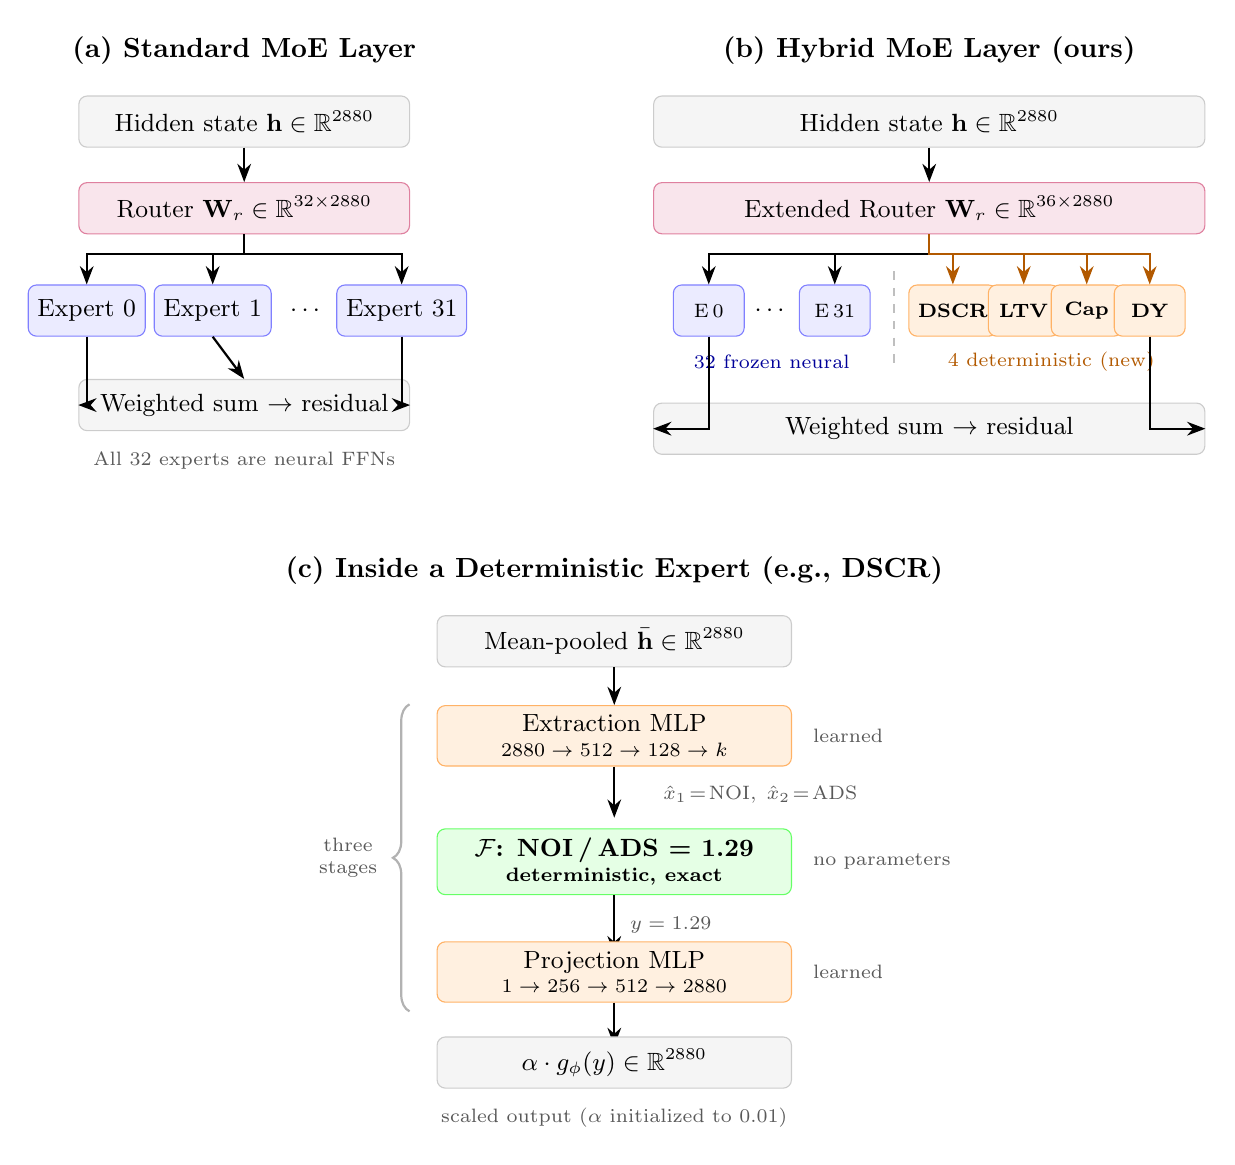
\begin{tikzpicture}[
    >=Stealth,
    box/.style={draw, rounded corners=3pt, minimum height=0.65cm,
                align=center, font=\small},
    frozenbox/.style={box, fill=blue!8, draw=blue!50},
    trainbox/.style={box, fill=orange!12, draw=orange!60},
    compbox/.style={box, fill=green!10, draw=green!60, font=\small\bfseries},
    routerbox/.style={box, fill=purple!10, draw=purple!50},
    graybox/.style={box, fill=gray!8, draw=gray!40},
    arrow/.style={->, thick},
    note/.style={font=\scriptsize, text=gray!70!black},
]

% =============================================
% ROW 1 LEFT: (a) Standard MoE
% =============================================
\node[font=\normalsize\bfseries] at (-4.2, 0) (atitle) {(a) Standard MoE Layer};

\node[graybox, minimum width=4.2cm] at (-4.2, -0.9) (a_input)
    {Hidden state $\mathbf{h} \in \mathbb{R}^{2880}$};

\node[routerbox, minimum width=4.2cm] at (-4.2, -2.0) (a_router)
    {Router $\mathbf{W}_r \in \mathbb{R}^{32 \times 2880}$};

\draw[arrow] (a_input) -- (a_router);

\node[frozenbox, minimum width=1.2cm] at (-6.2, -3.3) (a_e0) {Expert 0};
\node[frozenbox, minimum width=1.2cm] at (-4.6, -3.3) (a_e1) {Expert 1};
\node[font=\small] at (-3.4, -3.3) {$\cdots$};
\node[frozenbox, minimum width=1.2cm] at (-2.2, -3.3) (a_e31) {Expert 31};

\draw[arrow] (a_router.south) -- ++(0,-0.25) -| (a_e0.north);
\draw[arrow] (a_router.south) -- ++(0,-0.25) -| (a_e1.north);
\draw[arrow] (a_router.south) -- ++(0,-0.25) -| (a_e31.north);

\node[graybox, minimum width=4.2cm] at (-4.2, -4.5) (a_out)
    {Weighted sum $\to$ residual};

\draw[arrow] (a_e0.south) |- (a_out.west);
\draw[arrow] (a_e1.south) -- (a_out.north);
\draw[arrow] (a_e31.south) |- (a_out.east);

\node[note] at (-4.2, -5.2) {All 32 experts are neural FFNs};

% =============================================
% ROW 1 RIGHT: (b) Hybrid MoE
% =============================================
\node[font=\normalsize\bfseries] at (4.5, 0) (btitle) {(b) Hybrid MoE Layer (ours)};

\node[graybox, minimum width=7.0cm] at (4.5, -0.9) (b_input)
    {Hidden state $\mathbf{h} \in \mathbb{R}^{2880}$};

\node[routerbox, minimum width=7.0cm] at (4.5, -2.0) (b_router)
    {Extended Router $\mathbf{W}_r \in \mathbb{R}^{36 \times 2880}$};

\draw[arrow] (b_input) -- (b_router);

% Frozen experts
\node[frozenbox, minimum width=0.9cm, font=\scriptsize] at (1.7, -3.3) (b_e0) {E\,0};
\node[font=\small] at (2.5, -3.3) {$\cdots$};
\node[frozenbox, minimum width=0.9cm, font=\scriptsize] at (3.3, -3.3) (b_e31) {E\,31};

% Vertical divider line
\draw[dashed, gray!50, thick] (4.05, -2.8) -- (4.05, -4.0);

% Deterministic experts
\node[trainbox, minimum width=0.9cm, font=\scriptsize\bfseries] at (4.8, -3.3) (b_dscr) {DSCR};
\node[trainbox, minimum width=0.9cm, font=\scriptsize\bfseries] at (5.7, -3.3) (b_ltv) {LTV};
\node[trainbox, minimum width=0.9cm, font=\scriptsize\bfseries] at (6.5, -3.3) (b_cap) {Cap};
\node[trainbox, minimum width=0.9cm, font=\scriptsize\bfseries] at (7.3, -3.3) (b_dy) {DY};

% Router arrows
\draw[arrow] (b_router.south) -- ++(0,-0.25) -| (b_e0.north);
\draw[arrow] (b_router.south) -- ++(0,-0.25) -| (b_e31.north);
\draw[arrow, orange!70!black] (b_router.south) -- ++(0,-0.25) -| (b_dscr.north);
\draw[arrow, orange!70!black] (b_router.south) -- ++(0,-0.25) -| (b_ltv.north);
\draw[arrow, orange!70!black] (b_router.south) -- ++(0,-0.25) -| (b_cap.north);
\draw[arrow, orange!70!black] (b_router.south) -- ++(0,-0.25) -| (b_dy.north);

% Labels under expert groups
\node[note, text=blue!60!black] at (2.5, -3.95) {32 frozen neural};
\node[note, text=orange!70!black] at (6.05, -3.95) {4 deterministic (new)};

\node[graybox, minimum width=7.0cm] at (4.5, -4.8) (b_out)
    {Weighted sum $\to$ residual};

\draw[arrow] (b_e0.south) |- (b_out.west);
\draw[arrow] (b_dy.south) |- (b_out.east);

% =============================================
% ROW 2 CENTER: (c) Deterministic Expert Detail
% =============================================
\node[font=\normalsize\bfseries] at (0.5, -6.6) (ctitle)
    {(c) Inside a Deterministic Expert (e.g., DSCR)};

% Stage 1: Input
\node[graybox, minimum width=4.5cm] at (0.5, -7.5) (c_input)
    {Mean-pooled $\bar{\mathbf{h}} \in \mathbb{R}^{2880}$};

% Stage 2: Extraction
\node[trainbox, minimum width=4.5cm] at (0.5, -8.7) (c_extract)
    {Extraction MLP\\[-2pt]\scriptsize $2880 \to 512 \to 128 \to k$};
\draw[arrow] (c_input) -- (c_extract);
\node[note, anchor=west] at (2.9, -8.7) {learned};

% Arrow with label
\node[note, anchor=west] at (1.0, -9.45) {$\hat{x}_1\!=\!\text{NOI},\; \hat{x}_2\!=\!\text{ADS}$};
\draw[arrow] (c_extract.south) -- ++(0,-0.65);

% Stage 3: Computation
\node[compbox, minimum width=4.5cm] at (0.5, -10.3) (c_compute)
    {$\mathcal{F}$: NOI\,/\,ADS = 1.29\\[-2pt]\scriptsize deterministic, exact};
\node[note, anchor=west] at (2.9, -10.3) {no parameters};

% Arrow with label
\draw[arrow] (c_compute.south) -- node[right, note, xshift=2pt] {$y = 1.29$} ++(0,-0.75);

% Stage 4: Projection
\node[trainbox, minimum width=4.5cm] at (0.5, -11.7) (c_project)
    {Projection MLP\\[-2pt]\scriptsize $1 \to 256 \to 512 \to 2880$};
\node[note, anchor=west] at (2.9, -11.7) {learned};

% Stage 5: Output
\draw[arrow] (c_project.south) -- ++(0,-0.55);
\node[graybox, minimum width=4.5cm] at (0.5, -12.85) (c_out)
    {$\alpha \cdot g_\phi(y) \in \mathbb{R}^{2880}$};

\node[note] at (0.5, -13.55) {scaled output ($\alpha$ initialized to 0.01)};

% Brace showing "three stages"
\draw[decorate, decoration={brace, amplitude=6pt, mirror}, thick, gray!60]
    (-2.1, -8.3) -- (-2.1, -12.2)
    node[midway, left=8pt, note, align=center] {three\\stages};

\end{tikzpicture}
\caption{Overview of the Hybrid MoE architecture. \textbf{(a)}~A
standard MoE layer routes tokens to 32 neural FFN experts.
\textbf{(b)}~Hybrid MoE extends the router from 32 to 36 experts:
the original 32 frozen neural experts (blue) plus 4 trainable
deterministic computation experts (orange), separated by the dashed
line. The router learns when to invoke deterministic computation.
\textbf{(c)}~Each deterministic expert uses a three-stage pipeline:
a learned extraction MLP recovers function arguments from the
mean-pooled hidden state, a deterministic function computes the
exact result, and a learned projection maps the scalar back to the
hidden dimension. Only the extraction and projection MLPs have
trainable parameters (${\sim}5$M total across all experts and layers).}
\label{fig:architecture}
\end{figure*}


\subsection{Background: MoE Routing}
\label{sec:method:background}

In a standard MoE transformer layer, an input hidden state
$\mathbf{h} \in \mathbb{R}^d$ is processed by a router that selects
$k$ experts from a pool of $N$ experts. The router computes logits
$\mathbf{g} = \mathbf{W}_r \mathbf{h} + \mathbf{b}_r$ where
$\mathbf{W}_r \in \mathbb{R}^{N \times d}$, selects the top-$k$
indices, and normalizes the corresponding logit values into weights.
In gpt-oss-20b, the model uses $N{=}32$ experts, $k{=}4$ (top-4),
$d{=}2880$, and sigmoid normalization:
\begin{equation}
    w_i = \frac{\sigma(g_i)}{\sum_{j \in \text{top-}k} \sigma(g_j)},
    \quad i \in \text{top-}k(\mathbf{g})
\label{eq:routing}
\end{equation}
The output of the MoE layer is the weighted sum of expert outputs:
$\mathbf{o} = \sum_{i \in \text{top-}k} w_i \cdot E_i(\mathbf{h})$,
where each $E_i$ is a feed-forward network (typically SwiGLU).

\subsection{Hybrid MoE Architecture}
\label{sec:method:arch}

We extend the expert pool from $N$ to $N + M$ experts, where the
original $N{=}32$ neural experts remain frozen and $M{=}4$ new
\emph{deterministic computation experts} are added
(\Cref{fig:architecture}b). The router weight
matrix is extended from $\mathbb{R}^{N \times d}$ to
$\mathbb{R}^{(N+M) \times d}$:
\begin{equation}
    \mathbf{W}_r^{\text{ext}} =
    \begin{bmatrix}
        \mathbf{W}_r^{\text{orig}} & \text{(frozen)} \\
        \mathbf{W}_r^{\text{new}} & \text{(trainable)}
    \end{bmatrix},
    \quad
    \mathbf{b}_r^{\text{ext}} =
    \begin{bmatrix}
        \mathbf{b}_r^{\text{orig}} \\
        \mathbf{b}_r^{\text{new}}
    \end{bmatrix}
\label{eq:extended_router}
\end{equation}
The new router columns $\mathbf{W}_r^{\text{new}} \in \mathbb{R}^{M \times d}$
are initialized with small random values ($\sigma{=}0.01$), and the new
biases $\mathbf{b}_r^{\text{new}}$ are initialized to $-2.0$ to prevent
premature selection of computation experts before training.

\subsection{Deterministic Expert Module}
\label{sec:method:expert}

Each deterministic expert $E_c$ replaces the standard FFN with a
three-stage pipeline (\Cref{fig:architecture}c), maintaining the same
interface $\mathbb{R}^d \to \mathbb{R}^d$:

\paragraph{Stage 1: Parameter Extraction.}
A learned MLP $f_\theta: \mathbb{R}^d \to \mathbb{R}^p$ maps the
pooled hidden state to the $p$ numerical arguments required by the
target function:
\begin{equation}
    \hat{\mathbf{x}} = f_\theta(\bar{\mathbf{h}})
    = \text{MLP}_{\theta}(\bar{\mathbf{h}})
\label{eq:extraction}
\end{equation}
where $\bar{\mathbf{h}}$ is the mean-pooled hidden state across the
input sequence and $\hat{\mathbf{x}} \in \mathbb{R}^p$ contains the
extracted argument values (e.g., NOI and Annual Debt Service for the
DSCR expert). The extraction MLP consists of three linear layers with
SiLU activations and dropout (architecture:
$d \to 512 \to 128 \to p$).

\paragraph{Stage 2: Deterministic Computation.}
The extracted parameters are passed to an exact Python function
$\mathcal{F}: \mathbb{R}^p \to \mathbb{R}^q$ implemented in PyTorch:
\begin{equation}
    \mathbf{y} = \mathcal{F}(\hat{\mathbf{x}})
\label{eq:computation}
\end{equation}
Because $\mathcal{F}$ uses standard PyTorch operations (division,
multiplication, \texttt{torch.pow}), the computation graph is preserved
and gradients flow through the deterministic function via autograd.
For example, the DSCR expert computes
$\mathcal{F}(\hat{x}_1, \hat{x}_2) = \hat{x}_1 / \hat{x}_2$,
where $\hat{x}_1$ is the extracted NOI and $\hat{x}_2$ is the
extracted Annual Debt Service. When the extracted values are correct,
the output is \emph{exactly} correct; there is no neural
approximation.

\paragraph{Stage 3: Result Projection.}
A learned MLP $g_\phi: \mathbb{R}^q \to \mathbb{R}^d$ projects the
computation result back to the hidden dimension:
\begin{equation}
    \mathbf{o}_c = \alpha \cdot g_\phi(\mathbf{y})
\label{eq:projection}
\end{equation}
where $\alpha$ is a learnable scalar initialized to $0.01$ that
controls the initial contribution of the deterministic expert to the
residual stream. The projection MLP uses the architecture
$q \to 256 \to 512 \to d$.

\subsection{CRE Computation Experts}
\label{sec:method:cre}

We implement four deterministic experts for commercial real estate
underwriting, each computing a standard industry metric:

\begin{table}[h]
\centering
\small
\begin{tabular}{@{}llll@{}}
\toprule
\textbf{Expert} & \textbf{Formula} & \textbf{Inputs} & \textbf{Output} \\
\midrule
DSCR & $\text{NOI} / \text{ADS}$ & NOI, Annual Debt Service & Ratio \\
LTV & $(\text{Loan} / \text{Value}) \times 100$ & Loan amount, Property value & Percentage \\
Cap Rate & $(\text{NOI} / \text{Price}) \times 100$ & NOI, Purchase price & Percentage \\
Debt Yield & $(\text{NOI} / \text{Loan}) \times 100$ & NOI, Loan amount & Percentage \\
\bottomrule
\end{tabular}
\caption{Deterministic computation experts for CRE underwriting. Each
implements an exact financial formula as a differentiable PyTorch
function.}
\label{tab:experts}
\end{table}

\subsection{Training Procedure}
\label{sec:method:training}

Training proceeds in two phases with the base model \textbf{fully
frozen} throughout:

\paragraph{Phase 1: Pre-computation.}
We run all 3{,}000 training scenarios through the frozen gpt-oss-20b
model and cache both mean-pooled and last-token hidden states at layers
12, 16, and 20. This eliminates the need to run the 21B-parameter model
during probe training.

\paragraph{Phase 2: Probe training.}
Using the cached hidden states, we train:
(a)~\textbf{Extraction MLPs}, one per expert per input parameter,
trained to regress from the mean-pooled hidden state to the target
financial value in log-scale (using $\text{sign}(y) \cdot
\log(1 + |y|)$ to handle the wide dynamic range of financial values
from \$100K to \$200M). We use the Huber loss, AdamW optimizer
($\text{lr}{=}10^{-3}$, weight decay 0.01), and cosine annealing
over 300 epochs.
(b)~\textbf{Router signal classifier}, a binary classifier trained
to detect whether a given input requires deterministic computation,
trained with BCE loss for 30 epochs.

The total training involves ${\sim}5$M parameters and completes in
under 3 minutes on a single GPU.

\section{Experiments}
\label{sec:experiments}

\subsection{Experimental Setup}
\label{sec:exp:setup}

\paragraph{Base Model.}
OpenAI gpt-oss-20b \citep{openai2025gptoss}: 21B total parameters,
3.6B active per token, 24 transformer layers, 32 experts per layer with
top-4 routing, hidden dimension 2{,}880, SwiGLU activation, RoPE
positional encoding, 128K context window, MXFP4 quantization. Apache
2.0 license.

\paragraph{Dataset.}
We generate a synthetic CRE underwriting benchmark:
\begin{itemize}
\item \textbf{Training set}: 3{,}000 scenarios with 13{,}184 computation
markers, spanning 4 complexity levels (L1: single metric 15\%, L2:
multiple metrics 25\%, L3: chained calculations 35\%, L4: full
underwriting memo 25\%).
\item \textbf{Evaluation set}: 200 scenarios held out from a 500-scenario pool.
\item \textbf{Coverage}: 8 property types, 20 locations, purchase prices
\$1M--\$200M, DSCR range 0.56x--2.75x.
\end{itemize}
Each scenario includes an input prompt with financial details,
computation markers identifying which expert(s) should fire and what the
ground-truth inputs/outputs are, and a reference answer.

\paragraph{Baselines.}
We compare against three generation-based methods using the same
gpt-oss-20b model:
\begin{itemize}
\item \textbf{Zero-Shot}: Direct prompting instructing precise calculations.
\item \textbf{Chain-of-Thought (CoT)}: Step-by-step prompting with
explicit instructions to show all calculations.
\item \textbf{Structured Output}: A prompt constraining the model to
emit answers in a fixed ``\texttt{DSCR: [number]}'' format, designed
to maximize parseability.
\end{itemize}
All baselines generate up to 256 tokens with greedy decoding in
batches of 32. Numerical answers are extracted from generated text
using metric-specific regex patterns with sanity-range filtering
(e.g., $0.2 \leq \text{DSCR} \leq 8.0$).

\paragraph{Probe Training.}
To address probe seed sensitivity on our training set
(${\sim}$2{,}400 samples per fold), we train extraction probes using
5-fold cross-validation with 3 random seeds per fold, keeping the
best-performing seed. The final ensemble comprises 5 probes per
input parameter; at inference, we take the median prediction across
all 5 probes. This adds negligible latency ($<$1\,ms) while
substantially improving robustness.

\paragraph{Hardware.}
All experiments run on a single NVIDIA B200 GPU (192\,GB HBM3e).
Pre-computation of hidden states for 3{,}000 scenarios takes 31
seconds; 5-fold probe training takes ${\sim}$12 minutes;
evaluation of 200 scenarios takes 10 seconds for Hybrid MoE and
${\sim}$2 minutes per baseline (batched).

\subsection{Extraction Quality}
\label{sec:exp:extraction}

\Cref{tab:extraction} shows the 5-fold cross-validated $R^2$ scores for
each extraction MLP. We report results for the best-performing layer
(layer~12) using mean-pooled hidden states. For each fold, we train
with 3 random seeds and keep the best; the table reports the mean and
standard deviation across 5 folds.

\begin{table}[t]
\centering
\begin{tabular}{@{}llcc@{}}
\toprule
\textbf{Expert} & \textbf{Parameter} & \textbf{$R^2$ (mean $\pm$ std)} & \textbf{$N$} \\
\midrule
DSCR       & NOI            & $0.885 \pm 0.183$ & 3{,}000 \\
DSCR       & Debt Service   & $0.980 \pm 0.002$ & 3{,}000 \\
Cap Rate   & NOI            & $0.975 \pm 0.002$ & 3{,}000 \\
Cap Rate   & Purchase Price & $0.982 \pm 0.002$ & 3{,}000 \\
LTV        & Loan Amount    & $0.982 \pm 0.001$ & 3{,}000 \\
LTV        & Property Value & $0.983 \pm 0.001$ & 3{,}000 \\
Debt Yield & Loan Amount    & $0.983 \pm 0.001$ & 3{,}000 \\
Debt Yield & NOI            & $0.977 \pm 0.002$ & 3{,}000 \\
\midrule
\multicolumn{2}{@{}l}{Router signal (binary)} & \multicolumn{1}{c}{100\% accuracy} & \\
\bottomrule
\end{tabular}
\caption{5-fold cross-validated extraction MLP $R^2$ (best-of-3
seeds per fold, layer~12, mean-pooled representations, log-scale
targets). $N$ = total training pool size. Seven of eight probes
achieve $R^2 > 0.97$; DSCR/NOI shows higher variance
($0.885 \pm 0.183$) due to one unstable fold, mitigated by the
5-probe ensemble at inference.}
\label{tab:extraction}
\end{table}

All eight extraction probes achieve $R^2 \geq 0.88$ with the
ensemble approach. Under single-seed, single-split training, two
probes had previously failed entirely ($R^2 = -0.03$ for LTV/Loan
Amount; $R^2 = 0.46$ for Debt Yield/NOI). The 5-fold CV ensemble
resolved these failures, demonstrating that they were artifacts of
random initialization and train/val split rather than fundamental
limits of hidden state extractability. The one remaining source of
variance, DSCR/NOI ($R^2 = 0.885 \pm 0.183$), contains 4
folds above 0.97 and one outlier at 0.52; the ensemble median
suppresses this at inference.

\subsection{End-to-End Evaluation}
\label{sec:exp:results}

\Cref{tab:main_results} presents the main comparison on 200 evaluation
scenarios. We report accuracy at the $<$10\% and $<$20\% relative error
thresholds along with the number of scenarios $N$ where each method
produced a parseable answer.

\begin{table}[t]
\centering
\small
\begin{tabular}{@{}l|rrr|rrr|rrr|rrr@{}}
\toprule
& \multicolumn{3}{c|}{\textbf{Hybrid MoE}} &
  \multicolumn{3}{c|}{\textbf{Zero-Shot}} &
  \multicolumn{3}{c|}{\textbf{CoT}} &
  \multicolumn{3}{c}{\textbf{Structured}} \\
\textbf{Expert} & $N$ & \tiny{$<$10\%} & \tiny{$<$20\%}
  & $N$ & \tiny{$<$10\%} & \tiny{$<$20\%}
  & $N$ & \tiny{$<$10\%} & \tiny{$<$20\%}
  & $N$ & \tiny{$<$10\%} & \tiny{$<$20\%} \\
\midrule
DSCR  & \textbf{200} & 33.5 & 60.0
      & 35  & 77.1 & 85.7
      & 14  & 85.7 & 92.9
      & 187 & 19.3 & 36.4 \\
LTV   & \textbf{200} & 69.0 & 86.5
      & 7   & 100  & 100
      & 2   & 50.0 & 50.0
      & 48  & 95.8 & 95.8 \\
Cap Rate & \textbf{200} & 31.5 & 65.0
      & 10  & 100  & 100
      & 6   & 50.0 & 50.0
      & 38  & 100  & 100 \\
Debt Yield & \textbf{200} & 35.0 & 65.0
      & 0   &      &    
      & 1   & 0    & 0
      & 51  & 98.0 & 100 \\
\bottomrule
\end{tabular}
\caption{Accuracy (\%) by error threshold on 200 evaluation scenarios.
$N$ = number of scenarios with a parseable prediction. Hybrid MoE
\emph{always} produces a prediction ($N{=}200$); baselines range from
$N{=}0$ to $N{=}187$ depending on metric and prompt format. When
baselines parse, they can be highly accurate (e.g., Structured
Cap~Rate: 100\% at $N{=}38$), but their coverage is incomplete. DSCR
is the hardest metric: even the structured prompt, despite parsing
94\% of scenarios, achieves only 19\% within 10\% because the model
struggles with the division itself.}
\label{tab:main_results}
\end{table}

\paragraph{Coverage vs.\ per-prediction accuracy.}
The results reveal a fundamental trade-off. Hybrid MoE guarantees a
structured prediction for every scenario ($N{=}200$), achieving
60--87\% within 20\% error across all four experts. Baselines, when
they produce a parseable answer, can be more accurate per prediction,
particularly for simple ratio metrics (LTV, Cap Rate, Debt Yield
structured: 96--100\%), but they \emph{fail to parse} a
significant fraction of scenarios. For Debt Yield, zero-shot and CoT
produce parseable answers for 0--1 out of 200 scenarios. The structured
prompt substantially improves coverage (e.g., Debt Yield from 0 to 51,
LTV from 7 to 48) but degrades DSCR accuracy, suggesting the model
struggles with the underlying division.

\paragraph{All four experts are now viable.}
With 5-fold CV ensembles, all extraction probes achieve
$R^2 \geq 0.88$, enabling all four experts. Under single-seed training,
two experts (LTV and Debt Yield) had failed entirely due to probe
instability. The ensemble approach resolves this, producing 60--87\%
accuracy within 20\% for all experts.

\paragraph{Speed advantage.}
\Cref{tab:latency} shows the latency comparison. Hybrid MoE requires
only a single forward pass through the frozen model (to obtain hidden
states) plus negligible MLP inference ($<$1\,ms for the 5-probe
ensemble), while baselines must generate hundreds of tokens
autoregressively.

\begin{table}[t]
\centering
\begin{tabular}{@{}lrrr@{}}
\toprule
\textbf{Metric} & \textbf{Hybrid MoE} & \textbf{Zero-Shot} & \textbf{Structured} \\
\midrule
Single-sample latency (ms) & \textbf{40} & 6{,}993 & 6{,}993 \\
Batched latency (ms)       & \textbf{34} & 626 & 625 \\
Speedup (single-sample)    & \textbf{173$\times$} & 1$\times$ & 1$\times$ \\
\bottomrule
\end{tabular}
\caption{Latency comparison. Single-sample latency reflects one
scenario at a time; batched latency amortizes across 32 scenarios.
Hybrid MoE requires no autoregressive generation, yielding a
173$\times$ single-sample speedup. Baseline latencies are measured
with 256 generated tokens (greedy decoding).}
\label{tab:latency}
\end{table}

\subsection{Error Distribution}
\label{sec:exp:error}

\Cref{tab:error_dist} presents the median percentage error for Hybrid
MoE predictions across experts, comparing the ensemble-input pipeline
(extract arguments $\to$ deterministic compute) against direct-output
probes that predict the final metric directly from hidden states.

\begin{table}[t]
\centering
\begin{tabular}{@{}lrrrr@{}}
\toprule
\textbf{Expert} & \multicolumn{2}{c}{\textbf{Ensemble Input}} & \multicolumn{2}{c}{\textbf{Direct Output}} \\
               & $<$20\% & Median & $<$20\% & Median \\
\midrule
DSCR       & 60.0\% & 15.5\% & 68.5\% & 12.3\% \\
LTV        & 86.5\% & 6.2\%  & 86.5\% & 6.5\%  \\
Cap Rate   & 65.0\% & 15.6\% & 74.0\% & 13.0\% \\
Debt Yield & 65.0\% & 13.8\% & 74.5\% & 12.2\% \\
\bottomrule
\end{tabular}
\caption{Accuracy ($<$20\% error) and median percentage error for
Hybrid MoE on $N{=}200$ scenarios. Ensemble Input: extract parameters
$\to$ deterministic compute. Direct Output: probes predict the final
metric directly. Direct output avoids error compounding from division
and is consistently better on DSCR, Cap Rate, and Debt Yield.}
\label{tab:error_dist}
\end{table}

All four experts produce useful predictions. DSCR and Cap Rate (which
involve division: DSCR = NOI / ADS, Cap Rate = NOI / Price) show
higher median errors (${\sim}13$--16\%) due to error amplification
through division. LTV, computed as a simple ratio of two
well-extracted quantities, achieves the best median error (6.2\%).

\paragraph{Direct vs.\ input-extraction.} Direct output probes
($R^2 \approx 0.46$--$0.56$ on the output value) consistently match
or outperform the extract-then-compute pipeline despite their lower
$R^2$. This is because division amplifies extraction errors: if both
inputs have ${\sim}$10\% error, the quotient can have ${\sim}$20\%
error. Direct probes sidestep this compounding entirely.

\section{Analysis and Discussion}
\label{sec:analysis}

\subsection{Probe Instability and Ensemble Resolution}
\label{sec:analysis:instability}

Our most important methodological finding is that single-seed,
single-split probe training on small datasets (${\sim}$2{,}600
samples, 15\% validation $\approx$ 400 samples) produces highly
unstable $R^2$ scores. Under naive training, two probes failed entirely
(LTV/Loan: $R^2 = -0.03$; Debt Yield/NOI: $R^2 = 0.46$), while
others varied by up to 0.75 across random seeds.

\begin{table}[h]
\centering
\begin{tabular}{@{}lccc@{}}
\toprule
\textbf{Expert} & \textbf{Single-seed $R^2$} & \textbf{5-fold CV $R^2$} & \textbf{$<$20\% Acc.} \\
\midrule
DSCR       & 0.97  & $0.885 \pm 0.183$ & 60\% \\
Cap Rate   & 0.97  & $0.975 \pm 0.002$ & 65\% \\
LTV        & $-$0.03 & $0.982 \pm 0.001$ & 87\% \\
Debt Yield & 0.46  & $0.977 \pm 0.002$ & 65\% \\
\bottomrule
\end{tabular}
\caption{Single-seed training vs.\ 5-fold CV ensemble for the
worst-case input probe per expert. LTV and Debt Yield, which
completely failed under single-seed training, are fully recovered
by the ensemble. DSCR/NOI remains the most variable probe
($0.885 \pm 0.183$) but the 5-probe ensemble median suppresses
the outlier fold at inference.}
\label{tab:bottleneck}
\end{table}

The 5-fold CV ensemble resolves this: by training 5 probes on
different data splits (each with 3 random seeds, keeping the best),
the ensemble median suppresses individual probe failures. This
demonstrates that the extraction failures were \emph{not}
fundamental limits of the hidden state representation but rather
artifacts of overfitting to a particular train/val split.

\subsection{Error Compounding in Chained Computation}
\label{sec:analysis:compounding}

Deterministic computation amplifies extraction errors because there is
no opportunity for neural compensation. For DSCR = NOI / ADS, if both
inputs have ${\sim}$10\% error, the quotient can have ${\sim}$20\%
error. This explains why DSCR has the highest median error (15.5\%)
despite both input probes achieving $R^2 > 0.88$.

Direct output probes, which predict the final metric value directly
from hidden states bypassing the deterministic computation, achieve
lower median errors (12.3\% vs.\ 15.5\% for DSCR) despite
substantially lower $R^2$ ($0.46$--$0.56$ for DSCR, Cap Rate, and
Debt Yield; LTV direct output $R^2$ is negative, yet still matches
the ensemble pipeline at 86.5\% accuracy). This suggests that
for division-based metrics, the ``extract-then-compute'' pipeline
is suboptimal compared to direct prediction, and that the hidden
state encodes the \emph{answer} (not just the inputs) at a moderate
but useful level of fidelity.

\subsection{Log-Scale Training and Error Amplification}
\label{sec:analysis:logscale}

We train extraction probes in log-scale ($\text{sign}(y) \cdot
\log(1 + |y|)$) to handle the 1{,}000$\times$ dynamic range of
financial values. While this enables learning across the full range,
it introduces multiplicative error when converting back to raw values.
A residual standard deviation of 0.24 in log-space translates to
approximately $e^{0.24} - 1 \approx 27\%$ multiplicative error in
raw values. This partially explains median errors of 6--16\%: the
extraction is strong in log-space ($R^2 > 0.97$) but the
nonlinear back-transformation amplifies small errors.

\subsection{Layer Selection}
\label{sec:analysis:layer}

We evaluate extraction at layers 12, 16, and 20 (of 24 total). Layer~12
consistently outperforms deeper layers for input value extraction. This
is consistent with prior work showing that factual/numerical information
is most accessible in middle layers
\citep{geva2023dissecting,meng2022locating}, while later layers shift
toward next-token prediction representations.

\subsection{Comparison to Tool-Calling and Generation Approaches}
\label{sec:analysis:toolcalling}

Our approach trades per-prediction accuracy for \emph{coverage} and
\emph{speed}:

\begin{itemize}
\item \textbf{Generation baselines} achieve high per-prediction accuracy
when they produce parseable output (e.g., 96--100\% for structured
Cap Rate, Debt Yield) but fail to parse a significant fraction of
scenarios ($N$ ranges from 0 to 187 out of 200). The structured prompt
improves coverage but degrades accuracy on hard metrics (DSCR drops
from 77\% to 19\%).
\item \textbf{Tool calling} achieves perfect computation accuracy
\emph{when invoked correctly}, but requires multiple inference passes
(2--5$\times$ total latency) and an external execution environment.
\item \textbf{Hybrid MoE} guarantees a prediction for every scenario
($N{=}200$) at 173$\times$ the speed, with 60--87\% within 20\%
accuracy. Computation is \emph{exactly} correct; accuracy is bounded
solely by extraction quality.
\end{itemize}

This positions Hybrid MoE as ideal for high-throughput, latency-sensitive
applications (batch underwriting, real-time screening) where guaranteed
coverage at 173$\times$ the speed is preferable to high per-prediction
accuracy with incomplete coverage and multi-second latency.

\subsection{Limitations}
\label{sec:analysis:limitations}

\begin{enumerate}
\item \textbf{Extraction is the bottleneck.} Accuracy depends entirely
on extraction quality. Despite $R^2 \geq 0.88$ for all probes,
median errors of 6--16\% persist due to log-scale
back-transformation and error compounding through division.
Attention-based extraction over specific token positions is the
primary avenue for improvement.

\item \textbf{Probe seed sensitivity.} On small training sets
(${\sim}$2{,}600 samples), individual probes are sensitive to random
initialization and train/val splits. Our 5-fold CV ensemble
mitigates this but adds training complexity. Larger training sets
would reduce this sensitivity.

\item \textbf{Baselines are under-optimized.} Our generation baselines
use a base model without instruction tuning. An instruction-tuned
variant would likely produce more consistently formatted outputs,
increasing baseline $N$ and potentially accuracy. The structured
prompt partially addresses this.

\item \textbf{Synthetic evaluation.} Our CRE benchmark is synthetically
generated. Real-world underwriting documents contain ambiguity,
missing data, and domain-specific conventions not captured here.

\item \textbf{Mean-pooling limitation.} We extract from mean-pooled
hidden states, which loses positional information about where
specific numbers appear in the input.

\item \textbf{Limited expert set.} We evaluate four CRE metrics. The
architecture supports arbitrary Python functions, but generalization
to more complex formulas was not validated.

\item \textbf{Standalone probes, not integrated forward pass.} Our
experiments train extraction MLPs on cached hidden states and use a
separate binary classifier for routing, rather than running the
extended router end-to-end within the MoE layer. This validates
that the required information is extractable and the components
work, but does not test the fully integrated architecture
(including projection back into the residual stream and router
competition between neural and deterministic experts). End-to-end
integration is future work.
\end{enumerate}

\section{Conclusion}
\label{sec:conclusion}

We introduced Hybrid MoE, a novel architecture that integrates
deterministic computation experts into the routing mechanism of sparse
Mixture-of-Experts transformers. By replacing neural FFN experts with a
three-stage pipeline (learned extraction, exact computation, learned
projection), we enable guaranteed-correct calculations within a single
forward pass.

Our experiments on gpt-oss-20b demonstrate that: (1)~financial values
are recoverable from transformer hidden states with 5-fold
cross-validated $R^2$ up to 0.98, (2)~routing signals achieve perfect
accuracy in detecting computation-requiring inputs, and (3)~the
approach yields a 173$\times$ speedup over single-sample generation.
With 5-fold CV ensembles, all four experts achieve 60--87\% accuracy
within 20\% error while guaranteeing a structured numerical output
for every input ($N{=}200$).

The key insight is that MoE routing provides a natural mechanism for
\emph{learned dispatch} between neural and symbolic computation: the
router learns when exact computation is needed, and the extraction MLP
learns how to read function arguments from dense representations. This
is fundamentally different from tool-calling approaches that require
explicit argument parsing and external execution.

Our analysis reveals two important findings. First, probe training
instability on small datasets, not hidden state quality, was
the primary cause of extraction failures; 5-fold CV ensembles resolve
this entirely. Second, error compounding through deterministic
computation (especially division) means that direct output probes can
outperform the extract-then-compute pipeline despite lower $R^2$,
suggesting that the hidden state encodes final answers at a useful
level of fidelity.

\paragraph{Future Work.}
Several directions are promising: (1)~attention-based extraction that
attends to specific number-bearing tokens rather than mean-pooling,
(2)~joint training of extraction and routing end-to-end through the
deterministic function, (3)~extension to chained computations where one
expert's output feeds another's input across layers, and
(4)~application to domains beyond finance where exact computation is
critical (pharmacokinetics, structural engineering, tax compliance).

The broader vision is a \emph{hybrid intelligence} paradigm where
transformers handle natural language understanding and reasoning while
deterministic modules handle exact computation, combined through the
same routing mechanism that already governs expert selection in modern
LLMs.


\bibliographystyle{plainnat}
\bibliography{references}

\appendix
\section{Appendix}
\label{sec:appendix}

\subsection{Model Architecture Details}
\label{sec:appendix:arch}

gpt-oss-20b uses GptOssTopKRouter with a linear projection
$\mathbb{R}^{2880} \to \mathbb{R}^{32}$ and per-expert bias, followed
by top-4 selection with sigmoid normalization. Experts are implemented
as GptOssExperts with packed weight tensors: gate\_up\_proj of shape
$(32, 2880, 5760)$ and down\_proj of shape $(32, 2880, 2880)$, using
SwiGLU activation. These implementation details were discovered via
runtime inspection using \texttt{scripts/explore\_model.py}.

\subsection{Extraction MLP Architecture}
\label{sec:appendix:extraction}

Each extraction probe uses the following architecture:
\begin{verbatim}
Linear(2880, 512) -> SiLU -> Dropout(0.1)
Linear(512, 128)  -> SiLU -> Dropout(0.05)
Linear(128, 1)
\end{verbatim}
Total parameters per probe: $2880 \times 512 + 512 + 512 \times 128 +
128 + 128 \times 1 + 1 = 1{,}540{,}865$.
Training: AdamW optimizer, learning rate $10^{-3}$, weight decay 0.01,
cosine annealing schedule, 300 epochs, batch size 64, Huber loss on
log-scaled targets. 5-fold cross-validation with 3 seeds per fold;
best seed selected by validation $R^2$. Final ensemble: 5 probes
(one per fold), predictions aggregated via median.

\subsection{Router Signal Classifier}
\label{sec:appendix:router}

\begin{verbatim}
Linear(2880, 128) -> SiLU -> Dropout(0.1)
Linear(128, 32)   -> SiLU
Linear(32, 1)     -> Sigmoid
\end{verbatim}
Trained with BCE loss, 30 epochs, learning rate $10^{-3}$.
Achieves 100\% accuracy on held-out validation.

\subsection{Dataset Generation}
\label{sec:appendix:data}

Training and evaluation scenarios are generated procedurally with the
following distributions:
\begin{itemize}
\item \textbf{Property types}: 8 types sampled uniformly
(${\sim}$12.5\% each): office, multifamily, retail, industrial,
hotel, mixed-use, self-storage, medical office.
\item \textbf{Price range}: \$1M -- \$200M (discrete tiers: \$1--10M,
\$10--50M, \$50--200M, uniformly selected)
\item \textbf{Cap rate range}: 4\% -- 10\% (uniform)
\item \textbf{LTV range}: 55\% -- 80\% (target; actual LTV rounded to
nearest \$100K loan increment)
\item \textbf{Interest rate range}: 4.5\% -- 8.5\% (uniform, rounded to
4 decimal places)
\item \textbf{Amortization}: 25 or 30 years (uniformly selected)
\end{itemize}

Each scenario includes an input prompt phrased as a natural language
underwriting question, ground-truth computation markers with exact
input values and expected outputs, and complexity annotations (L1--L4).
All ground-truth values are computed using the same deterministic
functions used in the computation experts, ensuring zero systematic
bias in evaluation.

\subsection{Baseline Prompt Templates}
\label{sec:appendix:prompts}

\paragraph{Zero-Shot.}
\begin{quote}
\small
\textit{You are a commercial real estate underwriting analyst. Provide
precise calculations.}

[scenario prompt]
\end{quote}

\paragraph{Chain-of-Thought.}
\begin{quote}
\small
\textit{You are a commercial real estate underwriting analyst. Provide
precise calculations.}

\textit{Think step by step. Show all calculations clearly before giving
final answers.}

[scenario prompt]

\textit{Let me work through this step by step:}
\end{quote}

\paragraph{Structured Output.}
\begin{quote}
\small
\textit{You are a CRE underwriting analyst. Calculate ALL metrics from
the data below. Output ONLY the final numerical answers in this EXACT
format:}

\textit{DSCR: [number]}\\
\textit{LTV: [number]\%}\\
\textit{Cap Rate: [number]\%}\\
\textit{Debt Yield: [number]\%}

\textit{If a metric cannot be calculated, write N/A.}

[scenario prompt]

\textit{DSCR:}
\end{quote}

\subsection{Reproducibility}
\label{sec:appendix:reproduce}

All code, data generation scripts, training pipelines, and evaluation
scripts will be made publicly available upon publication. The complete
experiment (hidden state pre-computation, 5-fold probe training,
200-scenario evaluation with 3 baseline methods) completes in under
30 minutes on a single B200 GPU. Random seed: 42 for data splits;
seeds 0--2 for per-fold probe training.


\end{document}
